\documentclass[conference]{IEEEtran}
\IEEEoverridecommandlockouts
% The preceding line is only needed to identify funding in the first footnote. If that is unneeded, please comment it out.
\usepackage{cite}
\usepackage{amsmath,amssymb,amsfonts}
\usepackage{algorithmic}
\usepackage{graphicx}
\usepackage{textcomp}
\usepackage{xcolor}
\usepackage{float}
\usepackage{cleveref}
\usepackage{epstopdf}


\usepackage[T1]{fontenc}
\usepackage[utf8]{inputenc}
\def\BibTeX{{\rm B\kern-.05em{\sc i\kern-.025em b}\kern-.08em
    T\kern-.1667em\lower.7ex\hbox{E}\kern-.125emX}}


\DeclareMathOperator{\atantwo}{atan2}



\begin{document}

\title{Aarhus University MSc Course Project  \\ Control of Mobile Robots (AY 2019-20)}

\author{\IEEEauthorblockN{S. L. Skovgaard}
\IEEEauthorblockA{\textit{dept. of Engineering (of Aff.)} \\
\textit{Aarhus Unitversity (of Aff.)}\\
Aarhus, Denmark \\
201401682@post.au.dk}}

\maketitle

\begin{abstract}

This document is the final project in the course Control of Mobile Robots. This final project focus on designing and implementing a PID-controller, that is able to control a Parrot Bebop 2 drone in real world lab environment and investing the influence the different controller parameter have. To accomplish this is it necessary to transform linear velocity and angular rates in Inertial coordinates into the drones body frames. The project consist of two tasks. The first task involve the UAV hovering in a specific point 1 meter above the ground while being exposed to disturbances. The second task involve the UAV flying in a square shape trajectory by visiting the way-points (0,0,1), (2,0,1), (2,2,1) and (0,2,1) with an arbitrary yaw angle. 
In both task are different controller parameters tested both individually and combined. The transformation of linear velocity in Inertial coordinates into the UAVs body frames were successfully implemented. The PID-controller were successfully implemented both in the simulation and in the real world lab environment. The different changes in controller parameter resulted in the expected behavior. 

\end{abstract}

\section{Introduction}

This paper will carry out the final project in Control of Mobile Robots course at Aarhus university. It will involve implementing a closed-loop basic controller (PID-controller) for the Parrot Bebop 2 drone using ROS and Sphinx as development tools, using the bebop\_autonomy package. This final project will involve testing the designed close-loop controller on a real drone in a Lab environment. The ROS package vicon\_bridge will be used to communicate with the drone in the lab. \\
The final project will involve two different tasks. In the first task will the drone start of by taking off and hovering one meters above the ground, and keep that position for a fixed amount of time. The implemented controller on the drone will then be tested by applying physical disturbances to the drone when hovering. 

In the second task will the drone visit 4 different way points with an arbitrary yaw angle.  
In both tasks will different controller values, to see if practice is consistent with theory. These two tasks will be described and evaluated upon individually. This paper will fist touch upon the the theory behind then walk though one task at a time and reflect on the results.

Attached is two appendix, one contains the code implemented for task 1 and task 2 and the second appendix contains additional result from the lab that will be referred to in the paper.   

\section{Theory}\label{theory}
\subsection{The Robot Operating System}
In order to develop software for robots in a structured and easy way, the robot operating system(ROS)\cite{ros} has been used for this project. ROS is based upon the subscriber-publisher pattern where nodes are able to publish data as topics and subscribe to specific topics. In this project a node has been developed that is a subscriber and publisher which enables the node to: gather data, make calculations using this data and the publish new data. Furthermore a another node has been made solely for the purpose of gathering data and displaying this data using different plots.

\subsection{PID-controller}
In the two tasks for this project is a PID-controller implemented to control the Parrot Bebop2 drone. PID stands for proportional-integral-derivative controller. The \textbf{proportional} part of the controller acts as a linear feedback control system in which error correction is applied with a constant value that gives a proportional relationship between the measured value and the desired value. An increase in the $K_p$ parameter will result in a decrease in rise time and steady-state error as the current error will have bigger influence on the controller output. The negative side effect of an increase of $K_p$ is an increase in overshoot and small decrease in settling time as current error first becomes negative after the goal has been reached. The proportional control algorithm can be express mathematically as:

\begin{equation}
P_{out} = K_p e(t) \label{eq1}
\end{equation}

Where $P_{out}$ is the output of the controller, $K_p$ is the controller parameter, $e(t)$ is the measured error value at a certain time t. 

The \textbf{integral} part of the controller doesn't only look at the actual error as the proportional part does but it also looks as at the past errors, and if the applied force isn't enough to bring the error to zero, the force will be increased as time passes. An increase in the $K_i$ parameter will result in a decrease in rise time as the accumulated errors result in higher control output and it eliminates the steady-state error over time. The negative side effect of an increase in $K_i$ is an increase in overshoot and settling time as accumulated error first becomes smaller after the goal has been reached. The integral control algorithm can be express mathematically as:

\begin{equation}
I_{out} = K_i \int_{t}^{0}  e(\tau) d\tau \label{eq2}
\end{equation}

Where $I_{out}$ is the output of the controller, $K_i$ is the controller parameter, $e(\tau)$ is the error values from time 0 to the present time t. 

The \textbf{derivative} part of the controller look at the slope of the error over time and multiplies the rate of change by the derivative gain. The derivative part of the controller has an insight in the "future", for example if the object is quickly approaching the target, then the slope of the error over time will be negative and the controller output will decrease making sure the object doesn't overshoot by a lot. An increase in the $K_d$ parameter will result in overshoot and settling time as the slope of the error over time will result in a negative values as the object comes closer to the goal. An increase in $K_d$ doesn't have any notable influence in the rise time or the steady-state error. The derivative control algorithm can be express mathematically as:

\begin{equation}
D_{out} = K_d \frac{de(t)}{dt} \label{eq3}
\end{equation}

Where $D_{out}$ is the output of the controller, $K_d$ is the controller parameter, $de(t)$ is the change in error and $dt$ is the change in time.

The by combining the three parts into a PID-controller it will be expressed mathematically as:
 
\begin{equation}
u(t) = K_p e(t)+ K_i \int_{t}^{0}  e(\tau) d\tau+K_d \frac{de(t)}{dt} \label{eq4}
\end{equation}

Where $u(t)$ is the controller output. 

\subsection{Coordinate transformation}
When working with unmanned aerial vehicles it is important to understand how the body of the aerial vehicle is oriented with respect to the earth.
The inertial frame is the earth-fixed set of axes that is used as an unmoving reference.  It is commonly known that the x-axis points north, the y-axis points east and the z-axis points below. This is also called North-East-Down (NED) reference frame. 
To move from the inertial frame to the body frame a sequence of rotations has to be performed. The sequence involve rotating the frame around one axis at the time. Before the first rotation the body reference coordinate matches that of the inertial frame. \\\\
\textit{First rotation: Yaw rotation}\\
The yaw rotation represents rotation about the z-axis by an angle $\psi$. This rotation generates a new coordinate frame where the z-axis of the body frame is aligned with the Z-axis of the inertial frame and x and y coordinate are rotated with the angle $\psi$. We call this transformation $T_\psi$. The rotation of inertial frame to $T_\psi$ frame is preformed be multiplying the vector by the rotation matrix see \cref{eq5} 

\begin{equation}
T_\psi=
\begin{bmatrix}
x_1\\
y_1\\
z_1 
\end{bmatrix}=
\begin{bmatrix}
cos(\psi) & sin(\psi) & 0\\
-sin(\psi) & cos(\psi) & 0 \\
0 & 0 & 1
\end{bmatrix}
\begin{bmatrix}
x_I\\
y_I\\
z_I 
\end{bmatrix}\label{eq5}
\end{equation}
\\\\
\textit{Second rotation: Yaw and Pitch rotation}\\
The second rotation involves rotating the newly generated frame $T_\psi$ Y-axis by an angle $\theta$. This rotation generates a new coordinate frame where the Y-axis of the new coordinate frame is aligned with the Y-axis of the $T_\psi$ frame and x and z coordinate are rotated with the angle $\theta$. This transformation is again performed by multiplying the vector by the rotation matrix see \cref{eq6}

\begin{equation}
T_\theta=
\begin{bmatrix}
x_2\\
y_2\\
z_2 
\end{bmatrix}=
\begin{bmatrix}
cos(\theta) & 0 & -sin(\theta)\\
0 & 1 & 0 \\
sin(\theta) & 0 & cos(\theta)
\end{bmatrix}
\begin{bmatrix}
x_1\\
y_1\\
z_1 
\end{bmatrix}\label{eq6}
\end{equation}
\\\\
\textit{Third rotation: Yaw, Pitch and Roll rotation}\\
The third rotation involves rotating the newly generated frame $T_\theta$ Y-axis by an angle $\phi$.
This rotation generates a new coordinate frame where the X-axis of the new coordinate frame is aligned with the X-axis of the $T_\theta$ frame and x and z coordinate are rotated with the angle $\phi$. We call this final frame the body frame. This transformation is again performed by multiplying the vector by the rotation matrix see \cref{eq7}
\begin{equation}
T_\phi=
\begin{bmatrix}
x_B\\
y_B\\
z_B 
\end{bmatrix}=
\begin{bmatrix}
1 & 0 & 0\\
0 & cos(\phi) & sin(\phi) \\
0 & -sin(\phi) & cos(\phi)
\end{bmatrix}
\begin{bmatrix}
x_2\\
y_2\\
z_2 
\end{bmatrix}\label{eq7}
\end{equation}
\\
The complete rotation matrix for moving from the inertial frame to the body frame is given by \cref{eq8}
\begin{equation}
T^B_I = T_\psi T_\theta T_\phi\label{eq8}
\end{equation}
\\\\
\textit{Angular velocity of the UAV}\\
Since $\dot{\psi}$ is measured in the inertial frame, and $\dot{\theta}$ is measured in the Frame 1, and $\dot{\phi}$ is measured in the Frame 2. Are the relationship between the roll rate-p, and the pitch rate-q and the yaw rate-r and the Euler rates $(\dot{\psi},\dot{\theta},\dot{\phi})$ as follows \cref{eq9} 

\begin{equation}
\begin{bmatrix}
p\\
q\\
r 
\end{bmatrix}=
\begin{bmatrix}
1 & 0 & -S_\theta\\
0 & C\phi & C_\theta S\phi \\
0 & -S\phi & C_\theta C_\phi
\end{bmatrix}
\begin{bmatrix}
\dot{\psi}\\
\dot{\theta}\\
\dot{\phi}
\end{bmatrix}\label{eq9}
\end{equation}

Where the letter S represents sin and the letter C represents cos \cite{b2}\cite{b3}
\newpage

\subsection{Gazebo}
Gazebo is simulation environment that works together with ROS and is therefore suitable as a simulation tool for this project. Parrot provides the Bebop2 UAV as a downloadable package for Gazebo and this package is used for this project.

\section{Python code}
The code used for this project is built using the rospy package which is a Python library. Roscpp is also available if C++ is preferred. 

As mentioned earlier in this article, ROS makes use of the publisher/subscribre pattern. A single node containing several classes have been made for this project. The classes are: p-controller, takeoff and plot\_maker. 

\textbf{controller:} The responsibility of controller is handle the calculations and navigation of the UAV. The error or the euclidean distance to the goal-coordinates is calculated by first calculating the distance in the x-plane then the y-plane and lastly the z-plane. This results in three different distances which all are used as the error in each axis. In the controller class is the PID-controller logic implemented, so the error and time in handled differently in each part of the algorithm. The product of the PID algorithm is used to set the velocity in each direction, x, y and z.

\textbf{Takeoff:} As the name suggests this class handles the takeoff. It's a simple class that makes sure the drone has performed a complete takeoff sequence and when this is done it no longer has any responsibility. 

\textbf{Plot\_maker:} This class subscribes to the same topic as the controller class, /vicon/. It stores all values obtained from the vicon bridge and when the UAV has done its task, displays a number of plots which will be discussed later in the article. 


\section{Results and discussion}


\subsection{Simulation results}
To verify that the controller behaves as expected and to ensure that the drone will not crash when testing in real life, the controller has been tested in simulation first. The behaviour should be more or less the same when testing in a real world scenario. The simulation tests covers both the hovering and waypoint scenario however, only the waypoint scenario will be shown in this report. The drone used for the simulation as well as in the real world is the Parrot bebop2 UAV.

The controller coefficients are set to: Kp = 0.1, Ki = 0.01 and Kd = 0.1 as these values resulted in a reasonably quick and stable controller. On \cref{fig:sim_pos} the x, y and z position of the drone can be seen. It shows nicely how the drone goes to each waypoint in a controlled manner with a acceptable level of overshoot.  

\begin{figure}[hbtp]
	\centering
	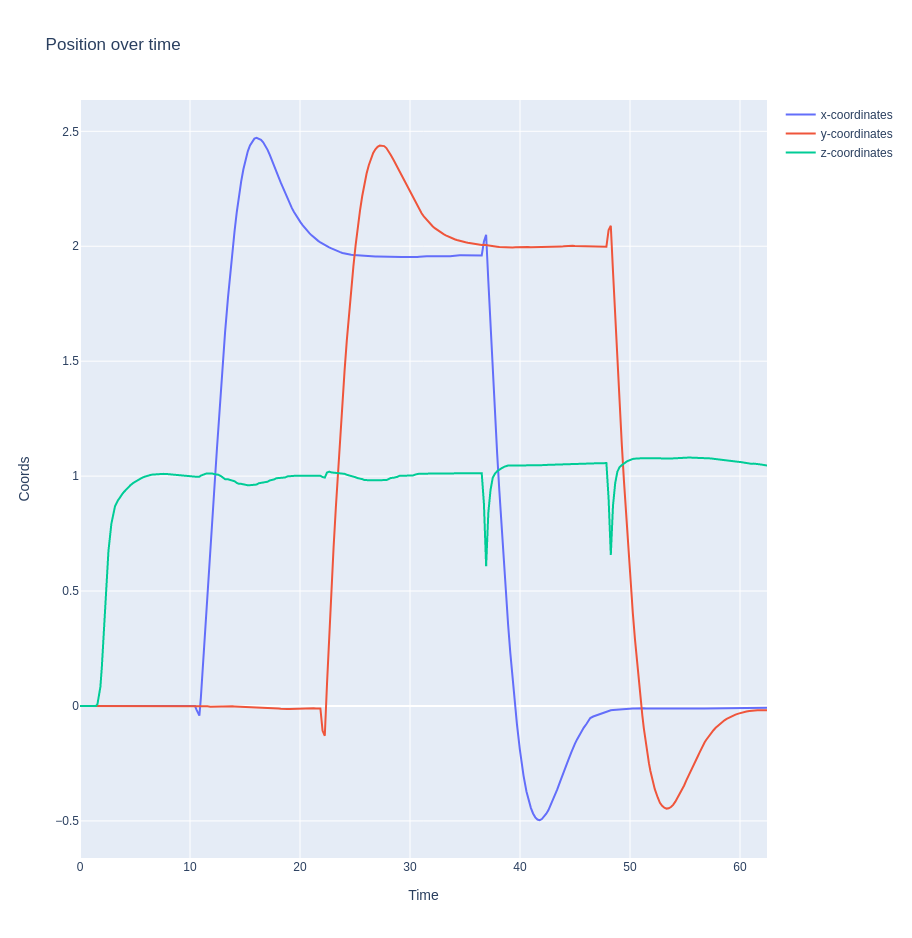
\includegraphics[width=1.0\linewidth]{images/task2_sim_pos.png}
	\caption{x, y and z coordinates of the drone in simulation. (Kp = 0.1, Ki = 0.01, Kd = 0.1)}
	\label{fig:sim_pos}
\end{figure}

Another way to visualize the simulation is using the program rviz which makes is possible to display the orientation as well as the position in 3D space. This can be seen on \cref{fig:sim_rviz}. On this figure it is also apparent that the yaw angle is constant for the drone at all times. 
After verifying that the drone is flying as intended in simulation real world testing can begin.

\begin{figure}[hbtp]
	\centering
	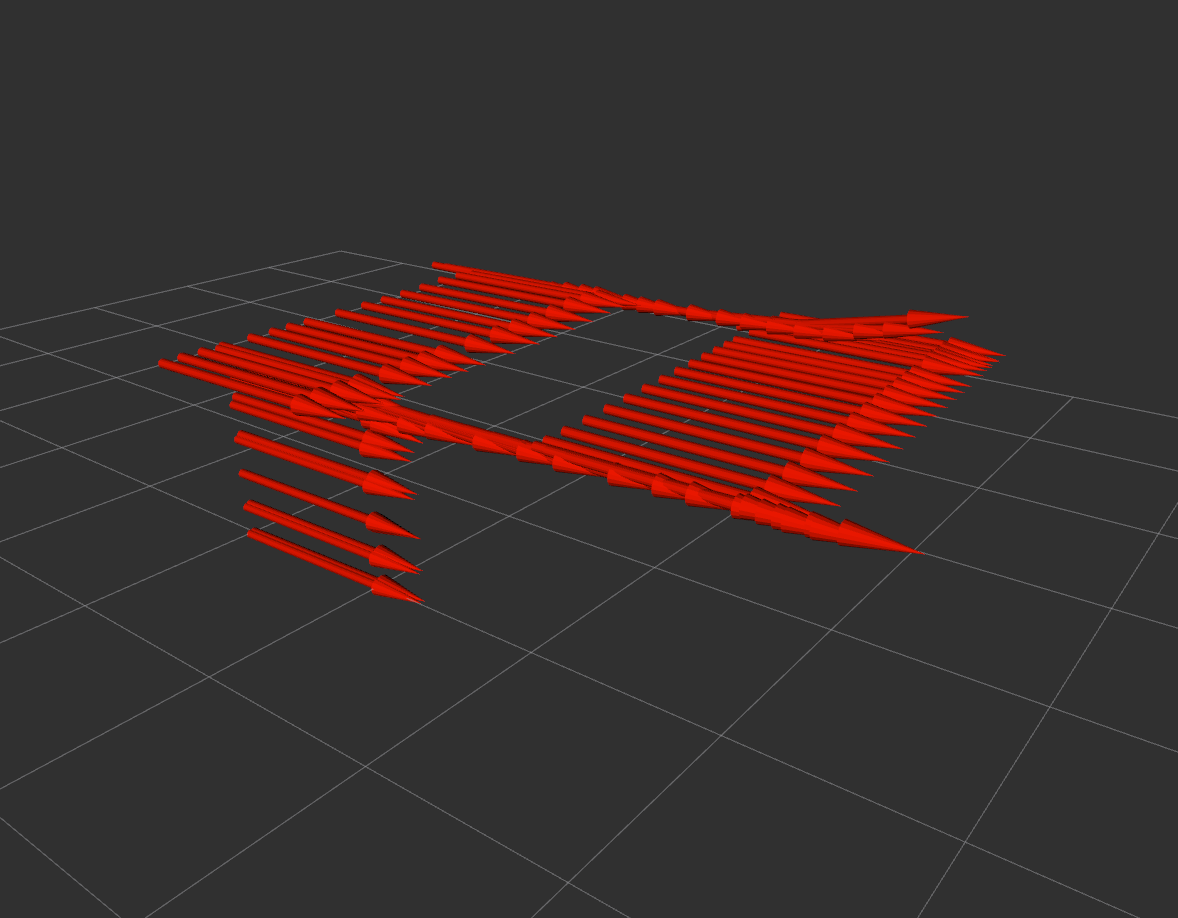
\includegraphics[width=1.0\linewidth]{images/task2_sim_rviz.png}
	\caption{x, y and z coordinates of the drone in simulation. (Kp = 0.1, Ki = 0.01, Kd = 0.1)}
	\label{fig:sim_rviz}
\end{figure}

\subsection{Real world results}
After having tested the controller in simulation the next step is to test it in a real world scenario. This is done using the Vicon motion control system which is able to accurately measure a UAV's position. This is done through 12 motion capture cameras that can locate small grey balls which are taped onto the drone itself. The Vicon system uses these balls as an reference point in space which can then be grouped together in the Vicon software and it will be able to publish the position as a topic in ROS.

\section{Conclusion}
The objective of this final project were to design and implement a PID-controller, that would be able to control a Parrot Bebop 2 drone in the real lab environment. To accomplish this was it necessary to transform linear velocity in inertial coordinates into the UAVs body frames. Another objective in this project were to investigate the influence of the different controller parameter both individually and combined and plot the results. 

This project are divided into two different tasks. The first task of the project involve the UAV hovering one meter above the ground at a specific point while being exposed to disturbances, which would make it possible to see the behavior of the controller. The second task of the project involve the UAV flying in square shape trajectory by visiting the way-points (2,0,1), (2,2,1), (0,2,1) and (0,0,1). The experiments of this project was carried out in real world setting at the AU Air lab located in Skejby. Both these tasks was carried out with different controller parameters, to investigate the influence of $K_p$, $K_i$ and $K_d$ individually and combined in a real world scenario. The PID-controller together with the transformation of linear velocity in Inertial coordinates into the UAVs body frames were successfully implemented.

The results showed that the theoretically influance of the controller parameter matched the physical results obtained at AU Air lab. The plots showed that an increase in $K_p$ resulted in lower rise time steady-state error but increase in overshoot and more unstable system. An increase in $K_i$ resulted in lower rise time and steady-state but an increase in overshoot of state-state error and more unstable system. Last an increase in $K_d$ resulted lower overshoot and settling time and better stability but an decrease in rise time. 


\begin{thebibliography}{00}

\bibitem{ros} http://wiki.ros.org/, date: 3/10/2020

\bibitem{Week3} Erdal Kaycan, ``Control Of Mobile Robots, week 3: Ground Robot models``, 16th of September 2020

\bibitem{book} RANDAL W. BEARD and TIMOTHY W. McLAIN, SMALL UNMANNED AIRCRAFT Theory and Practice, 2012

\bibitem{b2} CHRobotics, 2020, Understanding Euler Angles, http://www.chrobotics.com/library/understanding-euler-angles

\bibitem{b3} Control of Mobile Robots, Week 2 slides from lecture.

\end{thebibliography}
\vspace{12pt}

\end{document}
